\begin{figure}[!h]
    \centering
    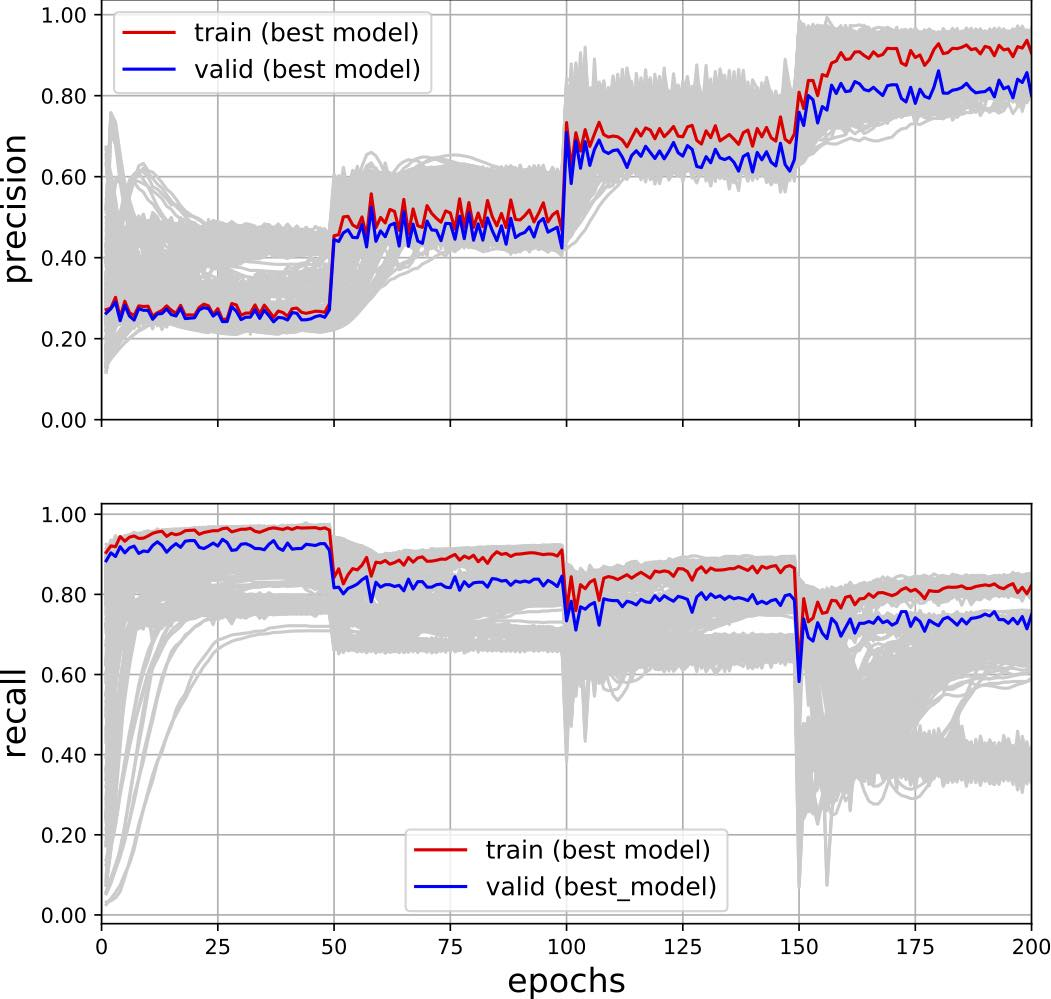
\includegraphics[width=0.8\textwidth,trim={0 0 0 0},clip]{content/chapters/false_alarm_control/figures/skorch_mlp_incremental_min_precision.jpg}
    \caption[Evidence of successful false-alarm-averse training of a model for MIMIC mortality risk prediction]{Evidence of successful false-alarm-averse training of a model for MIMIC mortality risk prediction. Every 50 epochs, the desired minimum precision $\alpha$ is stair-stepped up, beginning at 0.225, moving at 0.225 increments, and ending at 0.9. After each step, the model's empirical precision is quickly improved to approximately satisfy the desired $\alpha$ via gradient-based learning. Each gray line is one run from a random initialization, the best performing run (maximizing recall while satisfying our precision goals on training and validation) is highlighted in color.}
    \label{fig:mimic_precision_ramp_up}
\end{figure}